%% Public domain image from
%% http://www.public-domain-image.com/objects/computer-chips/slides/six-computers-chips-circuits.html
\renewcommand\chapterillustration{Math_transform/chapterImage}



\chapter{변환의 이해}
\index{변환}
\index{transformation}

수학적 의미에서 변환(transformation)이라는 것은 어떤 집합 $S$를 다른 어떤 집합 $S$로 대응시키는 함수이다. 
공간과 점, 그리고 벡터의 문제로 이해할 때, 변환이란 공간 상의 벡터나 점을 다른 벡터나 점으로 바꾸는 연산을 말한다.
어떤 벡터 $\mathbf a$가 $\mathbb R^{n}$에 속한다고 할 때,
이 벡터에 행렬 $\mathbf A \in \mathbb R^{n \times n}$을 곱하면 $\mathbf a$와 같은 차원의 벡터 $\mathbf b$를 얻는다.
즉,  $\mathbf b = \mathbf A \mathbf a ~ (\mathbf a, \mathbf b \in \mathbb R^n , \mathbf A \in \mathbb R^{n \times n})$.
이렇게 어떤 벡터를 동일한 차원의 다른 벡터로 옮기는 행렬 $\mathbf A \in \mathbb R^{n \times n}$을 변환행렬(transform matrix)라고 한다.
이 장에서는 3차원 벡터의 변환과 관련된 기본적인 수학 지식을 습득한다.

\section{좌표계의 이해}
\index{cooridnate system}\index{좌표계}

공간에 놓인 어떤 점의 위치는 다양한 좌표계를 이용하여 표현할 수 있다.
실시간 그래픽스에서 다루는 가장 일반적인 공간인 3차원을 이용하여 좌표계를 비교해 보자.

\subsubsection{직교 좌표계}
\index{직교 좌표계}\index{Cartesian coordinate}

일반적으로 가장 익숙한 좌표계는 직교좌표계이다. 이 좌표계는 데카르트 좌표계(Cartesian coordinate system)라고 부르기도 한다.
좌표는 3 개의 성분으로 이루어져 있으며, 각각의 성분은 세 개의 축 각각에 대해 점에서 수선을 내렸을 때에 수선의 발과 원점 사이의 거리가 된다.
직교 좌표계의 모습은 그림 \ref{fig:transform:CartesianCoord}에 나타나 있다.

\begin{figure}[h!]
  \centering
    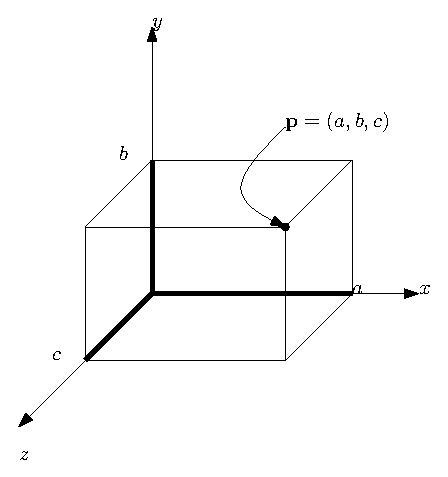
\includegraphics[width=8cm]{Math_transform/CartesianCoord.eps}
    \caption{직교 좌표계}
    \label{fig:transform:CartesianCoord}
\end{figure}

 \subsubsection{원기둥 좌표계}
\index{cylindrical coordinate}\index{원기둥 좌표계}

원기둥 좌표계(cylindrical coordinate system)은 어떤 좌표 $\mathbf p$를 표현할 때 이 좌표가 $xy$ 평면에서 얼마나 떨어져 있는지를 높이 $h$로 하고,
이 좌표와 $z$ 축 사이의 거리를 반지름 $r$로 표현한다. 점 $\mathbf p$는 이러한 높이와 반지름을 가진 원기둥의 상부 절단면의 원주에 놓여 있다.
원주에서 특정한 점을 지정하기 위해서는 기준선과 얼마의 각도를 이루고 있는지를 밝히면 된다. 이 각도를 $\theta$라고 하면, 원기둥 좌표계에서 하나의 점은
$(h, \theta, z)$로 표현된다. 이러한 좌표계의 모양은 그림 \ref{fig:transform:cylindricCoord}에 나타나 있다.

\begin{figure}[h!]
  \centering
    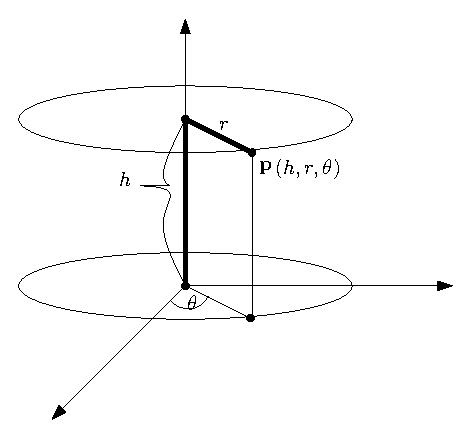
\includegraphics[width=8cm]{Math_transform/cylindricCoord.eps}
    \caption{원기둥 좌표계}
    \label{fig:transform:cylindricCoord}
\end{figure}

원기둥 좌표계로 $(r, z, \theta)$로 표현되는 좌표를 직교 좌표계로 옮기면 어떻게 될까.
그림 \ref{fig:transform:cyl2Cartesian}에서 보는 바와 같이 삼각함수를 이용하여 간단히 옮길 수 있다.
원기둥 좌표계의 좌표를 $\mathbf p_{cyl}$, 직교 좌표계의 좌표를 $\mathbf p_{cart}$으로 표현하면,
다음과 같이 변환이 가능하다.

$$(r, \theta, z)_{cyl} = ( r \cos \theta , r \sin \theta, z)_{cart}$$

\begin{figure}[h!]
  \centering
    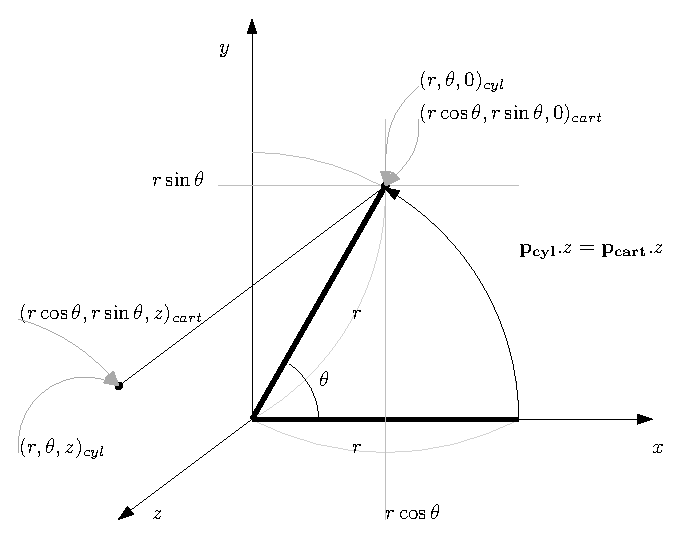
\includegraphics[width=8cm]{Math_transform/cyl2Cartesian.eps}
    \caption{원기둥 좌표계를 직교 좌표계로 변환하는 방법}
    \label{fig:transform:cyl2Cartesian}
\end{figure}

\subsubsection{구면좌표계}
\index{spherical coordinate}\index{구면 좌표계}

구면 좌표계(spherical coordinate system)은 어떤 좌표 $\mathbf p$를 지나며, 중심이 원점인 구면을 이용하여 좌표를 정의한다.
원점에서 이 점까지의 거리가 반지름 $r$이 된다.
반지름 $r$인 점 가운데  $x$ 축 위에 있는 점을 $\mathbf p_x$라고 하자. 이 점을 $xy$ 평면 위에서 거리 $r$을 유지한 채로 돌려
좌표 $\mathbf p$와 동일한 경도선 위에 놓이도록 회전시킬 때 필요한 각도를 $\phi$라고 하자. 그 이후 $z$축을 이 경도선을 따라 
회전시켜 점 $\mathbf p$를 지나도록 하는 데에 필요한 각도를 $\theta$라고 하자.
이제 좌표 $\mathbf p$는 반지름과 두 개의 각도로 $(r, \theta, \phi)$로 표현할 수 있다. 이러한 좌표계를 구면 좌표계라 한다.
구면 좌표계의 모양이 그림 \ref{fig:transform:sphericalCoord}에 나타나 있다.

\begin{figure}[h!]
  \centering
    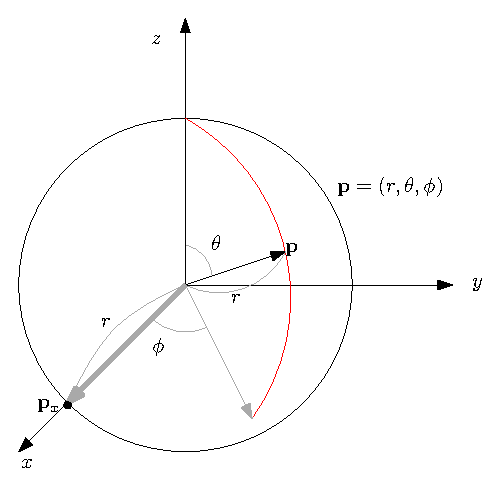
\includegraphics[width=8cm]{Math_transform/sphericalCoord.eps}
    \caption{구면 좌표계}
    \label{fig:transform:sphericalCoord}
\end{figure}

구면 좌표계를 사용할 때에는 각각의 성분이 될 수 있는 값들을 실수 전체로 사용하지 않고 일정한 범위로 제한을 하는 것이 일반적이다.
구면 좌표를 위와 같은 기하적 설명을 할 경우 다음과 같이 제한하는 것이 합리적이다 \cite{wiki:SphericalCoord_eng, wiki:SphericalCoord_kor}.
$$r \geq 0$$
$$0 \leq \theta \leq \pi$$
$$0 \leq \phi \leq 2 \pi $$

직교 좌표계의 좌표 $(x,y,z)$를 구면 좌표계로 옮길 때는 다음과 같은 계산을 수행한다\cite{wiki:SphericalCoord_eng, wiki:SphericalCoord_kor}.


\begin{eqnarray}
r &= \sqrt{x^2 + y^2 + z^2} \\ \nonumber
\theta & = \arccos \left ( \frac{z}{\sqrt{x^2 + y^2 + z^2}} \right ) \\ \nonumber
\phi &= \arctan \left ( \frac{y}{x} \right )
\end{eqnarray}

구면 좌표계의 좌표를 직교 좌표로 옮길 때에 수행하는 계산은 다음과 같다 \cite{wiki:SphericalCoord_eng, wiki:SphericalCoord_kor}.


\begin{eqnarray}
x &= r \sin \theta \cos \phi \\ \nonumber
y & = r \sin \theta \sin \phi \\ \nonumber
z & =r \cos \theta
\end{eqnarray}


\section{직교 좌표계에서의 변환}
\index{Cartesian coordinate!transformation}
\index{직교 좌표계!변환}

공간에 존재하는 점을 다룰 때에는 어떠한 좌표계를 사용해도 무방하다. 그런데, 컴퓨터 그래픽스 분야에서 가장 많이 사용되는 좌표계는 직교 좌표계이다.
본 절에서는 직교 좌표계를 기본적인 좌표계로 두고, 이 좌표계 내의 변환을 다루어 볼 것이다.

\subsection{어파인(affine) 변환}
\index{affine transformation}\index{어파인 변환}
\index{transformation!affine}\index{변환!어파인 변환}

게임을 구현하기 위한 3차원 그래픽스에서 흔히 사용되는 변환에는 다음과 같은 것들이 있다.

\begin{itemize}
\item 이동변환(translation)주어진 변위 벡터만큼 좌표를 동일하게 옮겨 놓는다.
\item 회전변환(rotation): 2차원에서는 기준점, 3차원에서는 기준축을 중심으로 주어진 각도만큼 돌아간다.
\item 크기변경(scaling): 각 축 방향으로 주어진 비율에 따라 좌표 값이 커지거나 줄어든다.
\end{itemize}

이러한 변환은 어파인 변환(affine transformation)의 일종인데, 어파인 변환은 서로 연결되어 있음을 의미하는 라틴어 `affinis'에서 온 말이다. 
어파인 변환은 직선 위의 점들을 직선을 유지한 상태로 변환하는 변환이며, 직선 위에서의 점들 사이의 거리 비가 변환된 직선 위에서 그대로 유지되는 변환이다. 
이런 특성에 의해 직선은 직선으로, 평행선은 평행선으로 유지된다. OpenGL이나 DirectX를 활용하는 실시간 컴퓨터 그래픽스에서는 여러 가지 효율성의 이유로
어파인 변환을 사용하는 것이 일반적이다. 

\section{이동변환(translation)}
\index{translation}\index{이동변환}
\index{transformation!translation}\index{변환!이동변환}
간단히 2차원을 먼저 생각해 보자. 이동변환은 어떤 좌표 $(x,y)$를 $x$ 축 방향으로 $a$ 만큼, $y$ 축 방향으로 $b$ 만큼 옮겨 놓는 일이다.
그림으로 표현하면 그림 \ref{fig:transform:translation}와 같다.
이때 $(a, b)$를 변위벡터(displacement vector)라고 할 수 있으며, 변환의 결과는 원래의 좌표에 변위 벡터를 더하여 얻을 수 있다.
즉, 이동 변환은 벡터 더학기로 표현할 수 있는 것이다.

$$(x', y') = (x,y) + (a,b) = (x+a, y+a)$$

3차원 공간의 좌표를 이동하는 것도 동일하다. 3차원 공간 뿐만 아니라, 모든 차원에 대해 다음과 같이 
벡터 $\mathbf a$를 변위 벡터 $\mathbf d$를 이용하여 $\mathbf x'$로 옮기는 이동 변환을 정의할 수 있다.

$$\mathbf a \in \mathbb R^n, \mathbf d \in \mathbb R^n$$
$$\mathbf x' = \mathbf a + \mathbf d$$
$$\mathbf x' \in \mathbb R^n$$

\begin{figure}[h!]
  \centering
    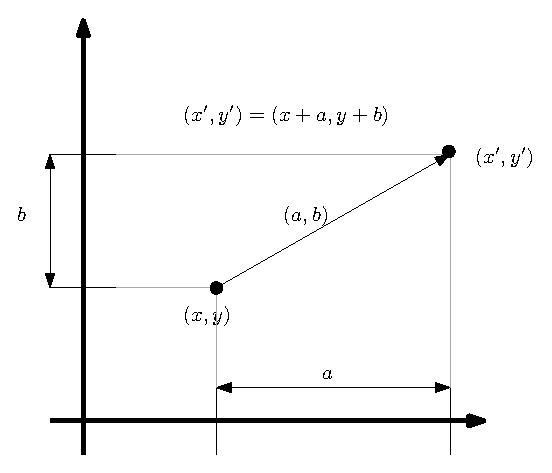
\includegraphics[width=8cm]{Math_transform/translation.eps}
    \caption{이동변환}
    \label{fig:transform:translation}
\end{figure}

\section{회전변환}
\index{rotation}\index{회전}
\index{transformation!rotation}\index{변환!회전변환}


여기서도 2차원의 경우를 먼저 살펴 보자.
2차원 평면에서 어떤 점이 회전하기 위해서는 회전의 중심이 되는 점이 필요하다. 이 점을 피벗(pivot)이라고 부르기도 한다.
어떤 점을 중심으로든 회전이 가능하지만 간략한 설명을 위해 원점을 회전의 중심으로 가정하자.
이것은 그림 \ref{fig:transform:rotation}에 나타난 $\mathbf p$를 원점을 중심으로 $\theta$ 만큼 회전하여 놓이는 지점 $\mathbf p'$를 구하는 문제가 된다.
원래의 좌표가 $(p_x,p_y)$일 때, $\theta$ 만큼 회전하여 얻는 $(p'_x, p'_y)$를 얻는 문제가 된다.

\begin{figure}[h!]
  \centering
    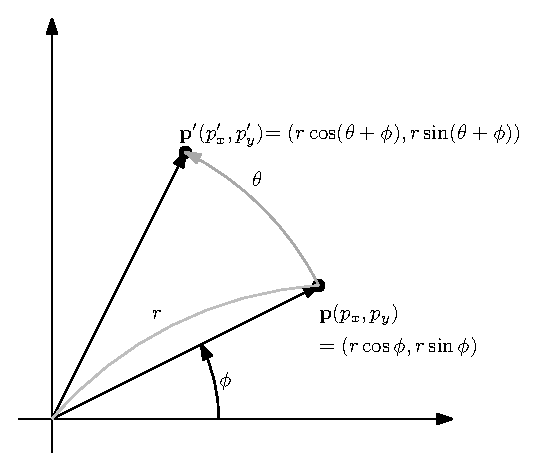
\includegraphics[width=8cm]{Math_transform/rotation.eps}
    \caption{2차원 회전 변환}
    \label{fig:transform:rotation}
\end{figure}

원점에서 원래의 좌표 $(p_x,p_y)$로 선분을 그으면, 이 선분은 어떤 길이 $r$과 $x$축과 이루는 각도 $\phi$를 가질 것이다.
좌표를 $(p_x,p_y)$는 반지름 $r$과 각도 $\phi$를 이용하여 다음과 같이 표현할 수 있다.

\begin{eqnarray}
p_x = r \cos \phi \\ \nonumber
p_y = r \sin \phi
\label{eq:positionWithTrigonometry}
\end{eqnarray}

이 좌표를 $\theta$만큼 회전하여 얻는 $(p'_x , p'_y)$는 $r$의 반지름과 $\phi+\theta$의 각을 가진 것으로 해석할 수 있다.
따라서 이 좌표는 다음과 같이 표현된다.

\begin{eqnarray}
p'_x = r \cos (\theta+ \phi) \\ \nonumber
p'_y = r \sin (\theta + \phi)
\label{eq:rotatedPointWithThetaAndPhi}
\end{eqnarray}


이것을 계산하려면 $\phi$를 먼저 계산해야 한다. 이러한 계산을 수행하지 않고, $p'_x$와 $p'_y$를 이미 알고 있는 $p_x$, $p_y$, 그리고 $\theta$를 이용하여
구할 수 있을까? 우선 다음과 같은 공식을 먼저 참조하자.

$$\cos (a+b) = \cos a \cos b - \sin a \sin b$$
$$\sin (a+b) = \sin a \cos b + \cos a \sin b$$

따라서 식 \ref{eq:rotatedPointWithThetaAndPhi}는 다음과 같이 다시 쓸 수 있다.

\begin{eqnarray}
p'_x = (r \cos \phi) \cos \theta - (r \sin \phi )\sin \theta \\ \nonumber
p'_y = (r \cos \phi) \sin \theta + (r \sin \phi )\cos \theta 
\label{eq:rotatedPointExtended}
\end{eqnarray}

식 \ref{eq:positionWithTrigonometry}를 고려하여 식 \ref{eq:rotatedPointExtended}를 다시 쓰면 다음과 같다.

\begin{eqnarray}
p'_x = p_x \cos \theta - p_y \sin \theta \\ \nonumber
p'_y = p_x \sin \theta + p_y \cos \theta 
\label{eq:rotatedPoint}
\end{eqnarray}

이러한 변환은 다음과 같은 행렬과 벡터의 곱으로 표현할 수 있다.

\begin{eqnarray}
\left [
\begin{array}{c}
p'_x \\ p'_y
\end{array}
\right ] =
\left [
\begin{array}{cc}
\cos \theta & - \sin \theta \\
\sin \theta & \cos \theta
\end{array}
\right ]
\left [
\begin{array}{c}
p_x \\
p_y
\end{array}
\right ]
\label{eq:rotationWithMatrixTransform}
\end{eqnarray}

이는 2차원 공간에서 어떤 점 $\mathbf p$를 원점 기준으로 $\theta$만큼 회전시켜 $\mathbf p'$를 얻는 변환은 회전변환 행렬 $\mathbf R(\theta)$을
이용하여 $\mathbf p' = \mathbf R(\theta) \mathbf p$로 표현할 수 있다는 것이다. 그리고 이 회전변환 행렬 $\mathbf R(\theta)$은 이미 살펴본 바와 같이
다음과 같이 표현된다.

\begin{eqnarray}
\mathbf R(\theta) = \left [ 
\begin{array}{cc}
\cos \theta & - \sin \theta \\
\sin \theta & \cos \theta
\end{array}
\right ]
\label{eq:rotationMatrix2D}
\end{eqnarray} 

\subsection{2차원 회전의 3차원 확장}

앞에서 살펴본 2차원 회전을 3차원 공간에서 살펴보면 회전 중심이 원점이 아니라 $z$ 축인 회전이 된다. 이를 바탕으로 3차원 회전 변환을 유도해 보자.

\subsubsection{$z$축 회전}

2차원 회전을 그대로 3차원에 적용하면 
3차원 공간의 점 $\mathbf p = (p_x, p_y, p_z)$을 $z$ 기준으로 회전하여 $\mathbf p' = (p'_x, p'_y, p'_z)$를 얻는 일이고,
이 변환은 2차원 변환가 큰 차이가 없이 $z$ 성분만 추가하면 된다.

이러한 변환은 다음과 같은 특성을 가진다.
\begin{itemize}
\item $z$ 축 성분은 그대로 유지된다. ($p'_z = p_z)$
\item $p_x, p_y$의 값은 2차원 회전과 동일하게 변환된다.
\end{itemize}

이것을 연립방정식 형태로 나타내면 다음과 같다.

\begin{eqnarray}
\begin{array}{clrrr}
p'_x  & = &\cos \theta \cdot p_x &- \sin \theta \cdot p_y &+ 0 \cdot p_z \\
p'_y  & = &\sin \theta \cdot p_x &+ \cos \theta \cdot p_y &+ 0 \cdot p_z \\
p'_z  & = & 0 \cdot p_x &+ 0 \cdot p_y &+ 1 \cdot p_z
\end{array}
\end{eqnarray}

이것은 다음과 같은 행렬 표현으로 다시 쓸 수 있다.

\begin{eqnarray}
\left [ \begin{array}{c} p'_x \\ p'_y \\ p'_z  \end{array} \right ] 
=
\left [ \begin{array}{rrr}
\cos \theta &- \sin \theta  & 0  \\
\sin \theta & \cos \theta  & 0 \\
0 & 0  & 1 
\end{array} \right ]
\left [ \begin{array}{c} p_x \\ p_y \\ p_z \end{array} \right ] 
\end{eqnarray}

\subsubsection{$y$축 회전}

\begin{figure}[h!]
  \centering
    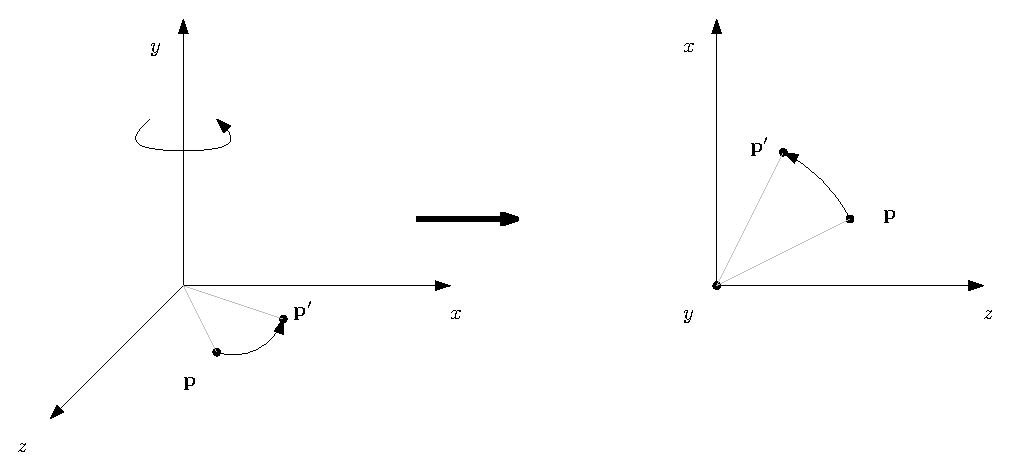
\includegraphics[width=15cm]{Math_transform/yAxisRotation.eps}
    \caption{$y$축 회전 변환}
    \label{fig:transform:yAxisRotation}
\end{figure}

$y$축을 기준으로 하는 회전은 그림 \ref{fig:transform:yAxisRotation}와 같다. 이것을 2차원 회전에 대응해 보면
3차원 $y$축 회전시의 $z$ 축은 2차원 회전의 $x$축에 해당하고, $x$ 축은 $y$축에 대응되는 것을 알 수 있다.
따라서, 다음과 같은 연립 방정식을 얻을 수 있다.

\begin{eqnarray}
\begin{array}{clrrr}
p'_z  & = &\cos \theta \cdot p_z &- \sin \theta \cdot p_x &+ 0 \cdot p_y \\
p'_x  & = &\sin \theta \cdot p_z &+ \cos \theta \cdot p_x &+ 0 \cdot p_y \\
p'_y  & = & 0 \cdot p_z &+ 0 \cdot p_x &+ 1 \cdot p_y
\end{array}
\end{eqnarray}

순서를 재배열하면 다음과 같은 식을 얻는다.
\begin{eqnarray}
\begin{array}{clrrr}
p'_x  & = & \cos \theta \cdot p_x &+ 0 \cdot p_y &+ \sin \theta \cdot p_z  \\
p'_y  & =  &0 \cdot p_x &+ 1 \cdot p_y & 0 \cdot p_z \\
p'_z  & = &-\sin \theta \cdot p_x &+ 0 \cdot p_y  & + \cos \theta \cdot p_z 
\end{array}
\end{eqnarray}

이것도 역시 행렬 표현으로 다시 쓸 수 있다.

\begin{eqnarray}
\left [ \begin{array}{c} p'_x \\ p'_y \\ p'_z  \end{array} \right ] 
=
\left [ \begin{array}{rrr}
\cos \theta & 0 &  \sin \theta  \\
0 & 1 & 0 \\
- \sin \theta & 0 & \cos \theta
\end{array} \right ]
\left [ \begin{array}{c} p_x \\ p_y \\ p_z \end{array} \right ] 
\end{eqnarray}

\subsubsection{$x$축 회전}

$x$축 회전은 그림 \ref{fig:transform:xAxisRotation}와 같이 가시화할 수 있으며, 여기서는 2차원 회전에서 $x$, $y$의 역할에
$y$와 $z$ 축이 각각 대응한다. 

\begin{figure}[h!]
  \centering
    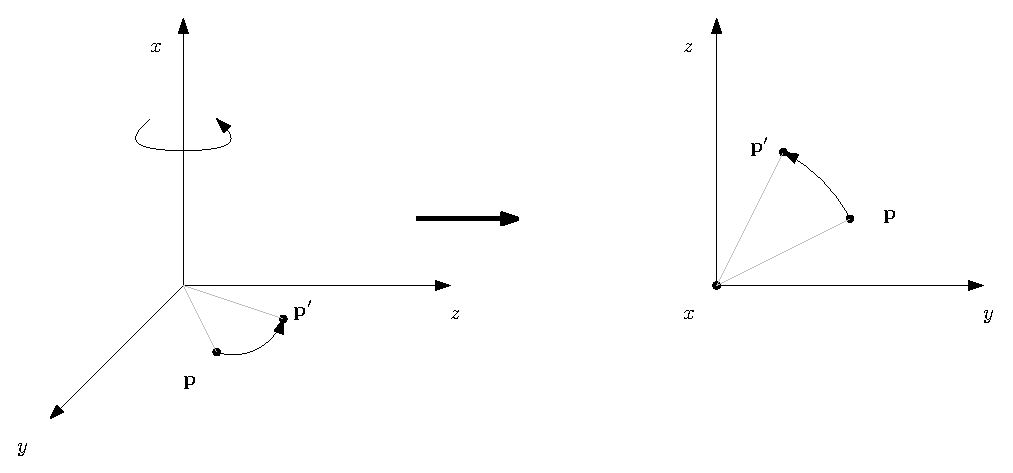
\includegraphics[width=15cm]{Math_transform/xAxisRotation.eps}
    \caption{$x$축 회전 변환}
    \label{fig:transform:xAxisRotation}
\end{figure}

이는 결국 다음과 같은 변환이 이루어짐을 의미한다.

\begin{eqnarray}
\begin{array}{clrrr}
p'_y  & = &\cos \theta \cdot p_y &- \sin \theta \cdot p_z &+ 0 \cdot p_x \\
p'_z  & = &\sin \theta \cdot p_y &+ \cos \theta \cdot p_z &+ 0 \cdot p_x \\
p'_x  & = & 0 \cdot p_y &+ 0 \cdot p_z &+ 1 \cdot p_x
\end{array}
\end{eqnarray}

이를 다시 배열하면 다음과 같다.

\begin{eqnarray}
\begin{array}{clrrr}
p'_x  & = & 1 \cdot p_x & + 0 \cdot p_y &+ 0 \cdot p_z  \\
p'_y  & = & 0 \cdot p_x & + \cos \theta \cdot p_y &- \sin \theta \cdot p_z \\
p'_z  & = & 0 \cdot p_x & + \sin \theta \cdot p_y &+ \cos \theta \cdot p_z  
\end{array}
\end{eqnarray}

행렬과 벡터의 곱으로 표현하면 다음과 같다.

\begin{eqnarray}
\left [ \begin{array}{c} p'_x \\ p'_y \\ p'_z  \end{array} \right ] 
=
\left [ \begin{array}{rrr}
1 & 0 & 0 \\
0 & \cos \theta & - \sin \theta \\
0 & \sin \theta & \cos \theta
\end{array} \right ]
\left [ \begin{array}{c} p_x \\ p_y \\ p_z \end{array} \right ] 
\end{eqnarray}


\subsubsection{3차원 회전행렬}
\index{rotation matrix}\index{회전변환 행렬}
\index{matrix!rotation}\index{행렬!회전변환}

지금까지의 내용을 정리하여 3차원 공간에서 $x$축, $y$축, 그리고 $z$축을 기준으로 $\theta$만큼의 회전을 일으키는 변환 행렬을
각각 $\mathbf R_x(\theta)$, $\mathbf R_y(\theta)$, $\mathbf R_z(\theta)$라고 하면 이들 행렬은 다음과 같다.

{\small
\begin{eqnarray}
\mathbf R_x(\theta)
=
\left [ \begin{array}{rrr}
1 & 0 & 0 \\
0 & \cos \theta & - \sin \theta \\
0 & \sin \theta & \cos \theta
\end{array} \right ]
~~~
\mathbf R_y(\theta)
=
\left [ \begin{array}{rrr}
\cos \theta & 0 &  \sin \theta  \\
0 & 1 & 0 \\
- \sin \theta & 0 & \cos \theta
\end{array} \right ]
~~~
\mathbf R_z(\theta)
=
\left [ \begin{array}{rrr}
\cos \theta &- \sin \theta  & 0  \\
\sin \theta & \cos \theta  & 0 \\
0 & 0  & 1 
\end{array} \right ]
\end{eqnarray}
}

\subsection{회전 행렬의 역행렬}
\index{회전행렬의 역행렬}
\index{정규직교 행렬}\index{orthonormal matrix}
\index{행렬!정규직교}\index{matrix!orthonormal}

지금까지 살펴본 모든 회전행렬은 특별한 특징을 가지고 있다.
회전 행렬을 구성하는 모든 열 벡터들을 살펴 보자.
우선 2차원 회전 행렬을 살펴보면, 첫 번째 열은 $(\cos \theta , \sin \theta)^{rm T}$이다.
이 열 벡터는 길이는 $\sqrt{ \cos^2 \theta + \sin^2 \theta}$이므로 1이다. 
두 번째 열의 길이 역시 $\sqrt{ \sin^2 \theta + \cos^2 \theta}$로 같다. 
즉 두 벡터 모두 단위 벡터이다. 그리고 이 두 벡터를 서로 내적하면
$\cos \theta ( - \sin \theta) + \sin \theta  \cos \theta $로 0이다. 이것은 이 두 벡터가 서로 직교함을 의미한다.
따라서 모든 벡터는 단위 벡터이고 서로 직교한다. 이러한 성질을 갖는 벡터들로 이루어진 행렬을 정규직교(orthonormal) 행렬이라고 한다.
정규직교 행렬의 역행렬은 그 행렬의 전치(transpose)와 같음이 이미 증명되어 있다.
따라서, 2차원 회전행렬의 역행렬은 이 행렬의 전치이다.

3차원 공간의 회전행렬들도 같은 방식으로 살펴보면, 모든 벡터가 단위 벡터이며 서로 직교함을 쉽게 확인할 수 있다.
따라서, 3차원 회전행렬 역시 역행렬을 구하려면 그 전치를 취하면 된다.

$${{\mathbf R}_x}^{-1}(\theta) = {{\mathbf R}_x}^{\rm T}(\theta)$$
$${{\mathbf R}_y}^{-1}(\theta) = {{\mathbf R}_y}^{\rm T}(\theta)$$
$${{\mathbf R}_z}^{-1}(\theta) = {{\mathbf R}_z}^{\rm T}(\theta)$$


\subsection{임의의 축에 대한 회전}

$x$, $y$, $z$ 축이 아닌 임의의 축에 대한 회전을 다소 복잡하다.
한가지 방법은 다음과 같은 순서의 작업을 수행하는 것이다.
임의의 회전축을 기준으로  $\theta$만큼 회전하는 변환은 다음과 같은 절차를 따라 구현할 수 있다.

\begin{enumerate}
\item 회전축이 원점을 지나도록 이동변환 $\mathbf T$를 적용한다.
\item 원점을 지나는 회전축이 $xz$ 평면에 놓이도록 $z$축 회전 $\mathbf R_1$를 적용한다.
\item 이 회전축이 $z$축과 동일한 방향이 되도록 $y$축 회전 $\mathbf R_2$를 적용한다.
\item $z$축을 기준으로 $\theta$만큼 회전하도록 $\mathbf R_z(\theta)$를 적용한다.
\item ${\mathbf R_2}^{-1}$, 즉 ${\mathbf R_2}^{\rm T}$를 적용한다.
\item ${\mathbf R_1}^{-1}$, 즉 ${\mathbf R_1}^{\rm T}$를 적용한다.
\item $\mathbf T^{-1}$, 즉 $- \mathbf T$를 적용한다.
\end{enumerate}

앞에서 우리는 이동 변환을 벡터의 더하기로 이해하였는데, 뒤에서 다룰 동차좌표계(homogeneous coordinate)을 이용하면
3차원 공간의 좌표는 4 개의 성분을 가진 벡터로 표현되고, 이동 변환과 회전 변환 모두 $4 \times 4$ 행렬로 표현하게 된다.
이 경우 위의 변환 절차는 모두 누적된 행렬의 곱으로 표현할 수 있고, 전체 변환을 하나의 행렬 $\mathbf R_{pivot}(\theta)$로 나타낼 수 있다.
이 행렬은 다음과 같다.

$$\mathbf R_{pivot}(\theta) = - \mathbf T {\mathbf R_1}^{\rm T} {\mathbf R_2}^{\rm T}  \mathbf R_z(\theta) \mathbf R_2  \mathbf R_1 \mathbf T $$

임의의 축을 기준으로 하는 회전을 다루는 데에 유용한 다른 방법은 사원수(quaternion)을 이용하는 것이다. 이것은 다른 장에서 다룰 것이다.

%% Public domain image from
%% http://www.public-domain-image.com/objects/computer-chips/slides/six-computers-chips-circuits.html
\renewcommand\chapterillustration{Math_transform/chapterImage}

\section{동차좌표계}
\index{동차좌표계}\index{homogeneous coordinate}
\index{사영기하학}\index{projective geometry}

동차좌표계(homogeneous coordinate)는 사영기하학(射影幾何學, projective geometry)에서 사용되는 좌표계로
$n$ 차원의 사영공간을 $n+1$의 좌표로 표현하는 좌표계이다.
사영기하학적 개념을 이해하는 것이 이 책의 목적이 아니므로 단순히 $n$ 차원 공간을 $n+1$ 개의 좌표로 표현한다는 정도의 개념으로 시작하자.
동차좌표계를 이용하면 컴퓨터 그래픽스의 문제를 다룰 때에 여러 가지 편리한 점이 있다. 그러한 이유로 실제 그래픽 API나 라이브러리들은
동차좌표계를 표준적인 좌표계로 채용하고 있다. 이 좌표계에 대한 이해를 해 보자.

\subsection{동차좌표계의 이해}
동차좌표계를 다루는 이유는 이 좌표계가 사영(projection)과 관련되어 있어 3차원 그래픽스에서 정의된 3차원 가상 공간 객체의 2차원 투영 이미지를 얻는 일과
유관하기 때문이며, 또 한 가지 이유는 3차원 공간의 어파인(affine) 변환들을 모두 $4 \times 4$의 행렬로 표현할 수 있기 때문이다.

단순히 숫자 하나를 추가하여 표현한다면 2차원 공간의 좌표 $(x,y)$는 $(x,y,1)$로 표현할 수 있을 것이다. 이렇게 벡터를 1행의 행렬처럼 표현할 경우,
이를 행벡터(row vector)라고 한다. 벡터를 다룰 때에는 행벡터보다 열벡터를 사용하는 경우가 많다. 우리도 열벡터로 표현할 것이다.
열벡터를 `하나의 열을 가진 행렬'로 이해한다면 앞의 좌표는 전치를 이용하여 $[x,y]^{\rm T}$와 $[x, y, 1]^{\rm T}$로 표현할 수 있다. (이 경우 행렬임을 강조하기 위해 둥근 괄호가 아니라 각진 괄호를 썼다.)

3차원 공간의 좌표를 표현하는 벡터 $[x,y,z]^{\rm T}$는 동차좌표계에서 $[x,y,z,1]^{\rm T}$로 표현할 수 있음을 쉽게 알 것이다.
보다 일반적인 형태는 마지막 숫자를 1이 아닌 다른 값도 가질 수 있는 것이다. 2차원 공간의 좌표와 3차원 공간의 좌표는 각각 다음과 같다.

$$[x,y,w]^{\rm T}, ~~~~~[x,y,z,w]^{\rm T}$$

\begin{figure}[h!]
  \centering
    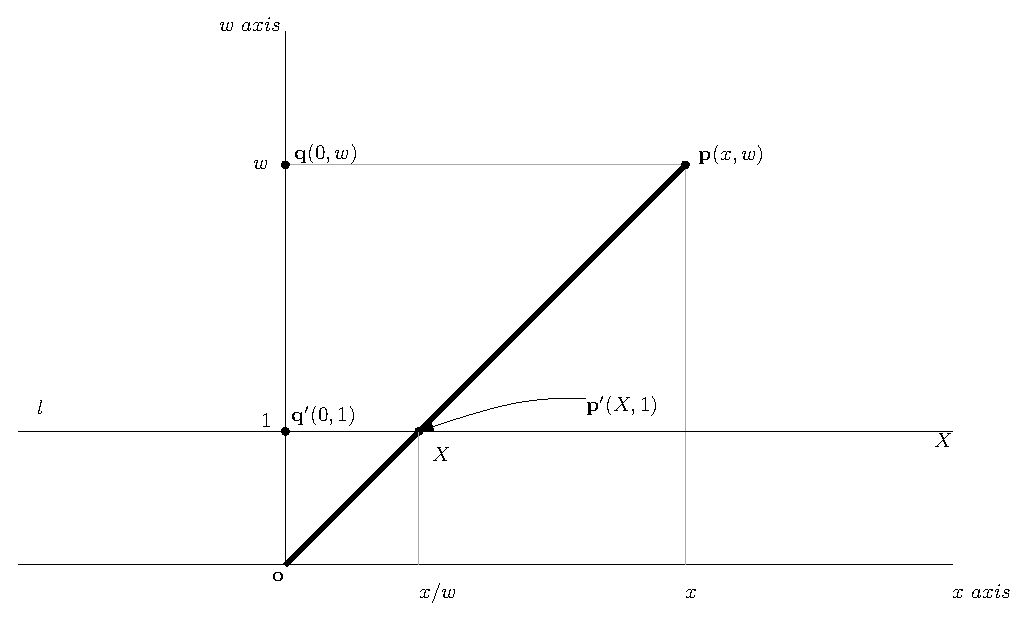
\includegraphics[width=12cm]{Math_transform/homogeneousConcept.eps}
    \caption{동차좌표계 이해를 위해 \cite{Ammeraal1986}에서 사용한 그림}
    \label{fig:transform:transformConcept}
\end{figure}

동차좌표계에 대한 직관적인 이해를 아메랄(Ammeraal)이 \cite{Ammeraal1986}를 통해 설명한 내용을 바탕으로 이해해 보자.
이 설명은 그림 \ref{fig:transform:transformConcept}를 이용하여 이루어질 것이다.
그림에는 두 개의 축이 있다. 하나는 $x$ 축이고, 다른 하나는 $w$ 축이다.
동차 좌표계에서 마지막 원소 $w$를 제외한 모든 성분은 이 $x$ 축 값으로 보면 되고, 마지막 원소는 이 $w$ 축 값이다.
$x$축 위에 있지 않는 점 $\mathbf p$는 중심 사영(central projection) $\mathbf p'$를 가지는데,
중심사영의 좌표는 $w=1$의 직선 $l$과 원점 $\mathbf o$에서 $\mathbf p$를 연결한 직선의 교차점이 된다.
이때 원점은 사영중심(center of projection)이 된다. 
이것은 $w$ 축과 $x$축을 모두 포함한 차원의 공간을 이보다 한 차원 낮은 $x$축 공간으로 떨어뜨리는 것과 같으며,
선분 $\overline{\mathbf o \mathbf p}$를 지나는 직선 위의 모든 점들이 이 $\mathbf p'$로 사영된다는 것이다.
이 점이 $(x,w)$라면 $\mathbf p'(X,1)$를 어떻게 구할 수 있는지 살펴 보자.
그림에서 닮은 삼각형 $\mathbf{opq}$와 $\mathbf{op'q'}$를 쉽게 찾을 수 있다.
삼각형 $\mathbf{op'q'}$를 보면 우리가 찾으려고 하는 $x$축 좌표 $X$는 $\overline{\mathbf{oq'}}$의 길이가 1이므로
이 길이와 $\overline{\mathbf{p'q'}}$ 길이의 비로 볼 수 있다.
$$X = \frac{X}{1} = \frac{|\mathbf{p'q'}|}{|\mathbf{oq'}|}$$

닮은 삼각형의 성질을 이용하여 이것이  ${|\mathbf{pq}|}/{|\mathbf{oq}|}$와 동일함을 알 수 있다.
그러므로 이 식은 다음과 같이 바뀐다.


$$X = \frac{X}{1} = \frac{|\mathbf{oq'}|}{|\mathbf{p'q'}|} = \frac{|\mathbf{oq}|}{|\mathbf{pq}|} = \frac{x}{w} $$


사영기하에서 $\mathbf {op}$를 지나는 직선 위의 모든 점들은 $(x,w)$ 형태의 좌표로 표현할 수 있고,
이 모든 점들은 $w=1$인 평면으로 중심사영을 수행했을 때, $w$ 좌표는 무의미해지면서 $(x/w)$의 좌표로 바뀌게 된다.
즉, 3차원 공간의 좌표를 표현하기 위해 동차좌표계를 사용한다면 $[x,y,z,w]^{\rm T}$의 형태가 되며,
이것은 위의 그림에서 $w$ 축을 포함한 공간이 된다. 이를 3차원 좌표로 바꾸는 것은 그림 \ref{fig:transform:transformConcept}에서
중심사영이 이루어지는 $w=1$ 평면으로 옮겨 놓는 것이고 이때의 좌표는 $[x/w,y/w,z/w]^{\rm T}$가 되는 것이다.
그리고 3차원 공간의 측면에서 보면, $\mathbf {op}$를 지나는 직선 위의 모든 점들이 동일한 점으로 간주되는 것이다.

\subsection{동차 좌표계 사용의 이점(利點)}
3차원 좌표 $[x,y,z]^{\rm T}$를 동차좌표계 좌표로 바꾸는 간단한 방법은 $w=1$ 평면에서의 좌표인 $[x,y,z,1]^{\rm T}$로 옮기면 된다.
여기에 어떤 이점이 있을까?
우선은 단순한 좌표 표현에서는 구분할 수 없었던 좌표와 벡터의 구분이 가능하다. $[x,y,z]^{\rm T}$가 3차원 좌표라면 이 좌표로 표현되는 지점은
3차원 공간내에 하나 밖에 없다. 하지만 이것이 벡터로 해석된다면 그것은 수 많은 동등 벡터를 표현하게 되며, 공간 내의 특별한 지점을 가리키지 않게 된다.
이 둘은 분명히 다르지만 단순한 좌표 표현 방식으로는 구분이 불가능하다.

동차 좌표계에서는 좌표와 벡터를 구분할 수 있다. 좌표는 $w \neq 1$인 $[x,y,z,w]^{\rm T}$이다. 3차원 공간 좌표로의 변환은 앞에서 본 바와 같이 
$[x/w, y/w, z/w]^{\rm T}$가 된다. 이때 $w$에 $k$를 곱했을 때, $x,y,z$에도 같은 $k$를 곱하면 모두 같은 3차원 좌표라고 할 수 있다.
$$[kx,ky,kz,kw]^{\rm T} = [x,y,z,w]^{\rm T}$$

이 $k$를 점점 0에 접근시켜도 여전히 같은 값을 가지는데, $k=0$인 경우에는 전혀 다른 의미가 된다.
이제 $w$ 좌표로 나누는 것이 불가능하다. 
이렇게 $w$축 값이 0인 경우는 어떻게 해석해야 할까? 이것은 벡터가 된다. 
$[x,y,z,0]^{\rm T}$는 위치를 가진 좌표 $[x,y,z]^{\rm T}$가 아니라 위치가 없는 벡터 $[x,y,z]^{\rm T}$가 된다.


동차좌표계의 또다른 이점은 앞에서 살펴본 이동변환와 회전변환을 모두 같은 차원의 행렬로 표현할 수 있다는 점이다.
우선 앞에서 다룬 변환들을 동차좌표계에서 다시 정의해 보자.

\subsubsection{동차좌표계에서의 이동변환}
\index{동차좌표계!이동변환}
\index{homogeneous coordiante!translation}

이동변환은 $[x,y,z]^{\rm T}$를 $\mathbf d=[d_x, d_y, d_z]^{\rm T}$만큼 이동하여 $[x+d_x, y+d_y, z+d_z]^{\rm T}$를 얻는 것이다.
이것을 동차좌표계로 표현하면 다음과 같다.

\begin{eqnarray}
\left [
\begin{array}{c}
x' \\y' \\ z' \\ 1
\end{array}
\right ]
=
\left [
\begin{array}{c}
x \\ y \\ z \\ 1
\end{array}
\right ]
+
\left [
\begin{array}{c}
d_x \\ d_y \\ d_z \\ 0
\end{array}
\right ]
=
\left [
\begin{array}{c}
x+d_x \\ y+d_y \\ z+d_z \\ 1
\end{array}
\right ]
\end{eqnarray}


이것은 동차좌표계를 도입하기 이전에 사용했던 벡터의 덧셈을 통해 이동변환을 표현하는 방식이다.
그런데, 동차좌표계에서는 이러한 이동변환을 다음과 같은 행렬 표현으로 바꿀 수 있다.


\begin{eqnarray}
\left [
\begin{array}{c}
x' \\y' \\ z' \\ 1
\end{array}
\right ]
=
\left [
\begin{array}{cccc}
1 & 0 & 0 & d_x \\
0 & 1 & 0 & d_y \\
0 & 0 & 1 & d_z \\
0 & 0 & 0 & 1 \\
\end{array}
\right ]
\left [
\begin{array}{c}
x \\ y \\ z \\ 1
\end{array}
\right ]
=
\left [
\begin{array}{c}
x+d_x \\ y+d_y \\ z+d_z \\ 1
\end{array}
\right ]
\end{eqnarray}

이제 이동변환을 행렬로 표현할 수 있게 되었다. 변위 벡터 $\mathbf d(d_x,d_y,d_z)$ 만큼의 이동을 수행하는 변환행렬을 $\mathbf T_{\mathbf d}$라고 하면
이동 변환은 다음과 같이 표현할 수 있다.

$$\mathbf p' = \mathbf T_{\mathbf d} \mathbf p, ~~~\mathbf T_{\mathbf d} \in \mathbb R^{4 \times 4}$$

이동변환 행렬 $\mathbf T_{\mathbf d}$의 역행렬은 어떻게 될까? 역행렬은 이 행렬이 일으킨 변환을 원래대로 되돌려 놓는 것이므로 
$\mathbf T_{- \mathbf d}$가 됨을 알 수 있다.

$$
\left [
\begin{array}{cccc}
1 & 0 & 0 & d_x \\
0 & 1 & 0 & d_y \\
0 & 0 & 1 & d_z \\
0 & 0 & 0 & 1 \\
\end{array}
\right ]^{-1}
= 
\left [
\begin{array}{cccc}
1 & 0 & 0 & -d_x \\
0 & 1 & 0 & -d_y \\
0 & 0 & 1 & -d_z \\
0 & 0 & 0 & 1 \\
\end{array}
\right ]
$$


\subsubsection{동차좌표계에서의 회전변환}
\index{동차좌표계!회전변환}
\index{homogeneous coordiante!rotation}
이제 동차좌표계에서 회전변환을 어떻게 표현할 수 있는지를 생각해 보자. 우선 3차원 공간에서 정의되었던 회전 변환을 $\mathbf R_{33}$이라고 하자.
동차좌표계에서의 하나의 좌표가 4 개의 성분을 가지므로 회전 행렬은 $\mathbb R^{4 \times 4}$에 속해야 한다. 이런 회전을 수행하는 회전행렬을 
$\mathbf R_{44}$라고 하자.

동차좌표계에의 회전을 구하려면
3차원 좌표 $\mathbf p(x,y,z)$가 $\mathbf R_{33}$에 의해 $\mathbf{p'}(x',y',z')$로 옮겨질때,
동차좌표계의 어떤 좌표가 $\mathbf p(x,y,z,1)$가 $\mathbf R_{44}$에 의해 회전하면 $\mathbf{p'}(x',y',z',1)$로 옮겨지게 하면 된다.
원소가 모두 0인 3차원 열벡터를 $\mathbf O_3^{col}$, 원소가 모두 0인 행벡터를 $\mathbf O_3^{row}$라고 하면,
$\mathbf R_{44}$를 다음과 같이 표현할 수 있다.

$$\mathbf R_{44} = 
\left [
\begin{array}{cc}
\mathbf R_{33} & \mathbf O_3^{col} \\
\mathbf O_3^{row} & 1
\end{array}
\right ]
$$

이제 동차좌표계에서 $x$축, $y$축, $z$축 기준 회전행렬을 다음과 같이 구할 수 있다.

$$
\mathbf R_{44}^x =
\left [
\begin{array}{cccc}
 1 & 0 & 0 & 0 \\
 0 & \cos \theta & -\sin \theta &  0\\
 0  & \sin \theta & cos \theta & 0 \\
 0 & 0 & 0 & 1 \\
\end{array}
\right ]
$$

$$
\mathbf R_{44}^y =
\left [
\begin{array}{cccc}
 \cos \theta & 0 & \sin \theta & 0 \\
 0 & 1 & 0 & 0 \\
- \sin \theta & 0  & \cos \theta & 0 \\
 0 & 0 & 0 & 1\\
\end{array}
\right ]
$$

$$
\mathbf R_{44}^z =
\left [
\begin{array}{cccc}
 \cos \theta & - \sin \theta & 0 & 0 \\
 \sin \theta  & \cos \theta & 0 & 0 \\
 0 & 0 & 1 & 0 \\
 0 & 0 & 0 & 1\\
\end{array}
\right ]
$$

\subsubsection{복합 변환}
\index{동차좌표계!복합 변환}
\index{homogeneous coordinate!composite transformation}

이제 변환행렬은 이동과 회전을 막론하고 누적할 수 있다.
좌표를 $\mathbf R_{44}$를 이용하여 회전하고, 이를 $\mathbf T_{\mathbf d}$ 만큼 이동하는 변환을 생각해 보자.
이 변환은 어떤 점 $\mathbf p$가 있다면, 다음과 같이 $\mathbf p'$를 구하는 것이다.

\begin{eqnarray}
\mathbf p' = \mathbf T_{\mathbf d} \mathbf R_{44}  \mathbf p
\label{eq:RotationAndTranslation}
\end{eqnarray}

앞에서의 정의와 함께 $3 \times 3$ 크기의 항등 행렬을 $\mathbf I_{33}$라고 하면 식 \ref{eq:RotationAndTranslation}은 다음과 같이 
다시 쓸 수 있다.

\begin{eqnarray}
\label{eq:RotationAndTranslation2}
\mathbf p' & = &
\left [
\begin{array}{cc}
\mathbf I_{33} & \mathbf d \\
\mathbf O_3^{row} & 1
\end{array}
\right ]
\left [
\begin{array}{cc}
\mathbf R_{33} & \mathbf O_3^{col} \\
\mathbf O_3^{row} & 1
\end{array}
\right ]
\mathbf p \\ \nonumber
& = &
\Large{
\left [
\begin{array}{cc}
\mathbf R_{33} & \mathbf d \\
\mathbf O_3^{row} & 1
\end{array}
\right ]
\mathbf p}
\end{eqnarray}

동차좌표계에서 어떤 변환이 회전과 이동으로만 이루어져 있다면 변환행렬의 좌측 상단 $3 \times 3$의 부분은 회전을 결정하고,
최우측 열은 이동변환의 변위를 결정하는 것이다.

식 \ref{eq:RotationAndTranslation2}에 나타난 행렬의 역행렬은 어떻게 구할 수 있을까?
가해진 변환을 역으로 수행할 것이므로, 
$\mathbf T_{-\mathbf d}$의 이동을 먼저 수행하고, ${\mathbf R_{33}}^{-1}$의 회전을 수행하면 된다.
앞서 설명한 바와 같이 정규직교 행렬의 경우 전치(transpose)가 역행렬이 된다. 회전행렬은 정규직교 행렬이기 때문에
$\mathbf R_{33}^{-1} = \mathbf R_{33}^{\rm T}$이다.

따라서 식 \ref{eq:RotationAndTranslation2}에 나타난 행렬의 역행렬은 다음과 같다.

\begin{eqnarray}
\label{eq:RotationAndTranslationInverse}
\left [
\begin{array}{cc}
\mathbf R_{33}^{\rm T} & \mathbf O_3^{col} \\
\mathbf O_3^{row} & 1
\end{array}
\right ]
\left [
\begin{array}{cc}
\mathbf I_{33} & \mathbf -d \\
\mathbf O_3^{row} & 1
\end{array}
\right ]
= 
\Large{
\left [
\begin{array}{cc}
\mathbf R_{33}^{\rm T} & - \mathbf R_{33}^{\rm T} \mathbf d \\
\mathbf O_3^{row} & 1
\end{array}
\right ]
}
\end{eqnarray}

동차좌표계 변환행렬이 있는데, 만약 $\mathbf R_{33}$ 부분이 정규직교가 아니라면, 이 행렬은 회전과 이동 이외에 크기변환 등이 추가되어 있는 것이다.

\section{좌표계의 변환}

어떤 점이 좌표계 $A$에 의해 $\mathbf p_A$라고 하자. 이 점을 다른 좌표계 $B$의 입장에서 보면 다른 좌표 $\mathbf p_B$가 된다.
이렇게 좌표계가 달라질 때 바뀐 좌표계에 따라 새로운 좌표를 계산하는 일은 그래픽스에서 매우 빈번히 나타나는 작업이다.


대표적인 경우가 가상 공간 내의 모든 객체의 위치를 하나의 기준으로 정의하는 데에 필요한 전역좌표계(global coordinate system)이며, 
다른 하나는 개별 객체 내에 정의된 지역좌표계(local coordinate system)이다. 
가상 공간에서 객체들이 이동, 회전 변환 등을 통해 위치와 방향이 바뀌어 있을 때, 이 객체를 구성하는 기하 정보의 좌표는 전역좌표계를 기준으로는 변경된다.
하지만, 이 객체가 변형을 일으키지 않는다면, 지역좌표계를 기준으로 한 기하정보는 언제나 일정하게 유지된다.

이 장에서는 좌표계가 변경되었을 때에 좌표가 어떻게 바뀌는지에 대해 살펴볼 것이다.

\subsection{좌표계의 이동}

좌표계가 그림 \ref{fig:transform:coordinateTranslate}에 나타난 바와 같이 일정한 변위 벡터 $\mathbf d$에 의해 이동(translate)했다고 하자.
이렇게 좌표계가 이동했을 때의 원래의 좌표계를 $A$, 옮겨간 좌표계를 $B$라고 하면 
어떤 하나의 점 $\mathbf p$가 각각의 좌표계에서 같는 좌표를 $\mathbf p_A$와 $\mathbf p_B$라고 하자.
두 좌표의 관계는 다음과 같다.

$$\mathbf p_A = \mathbf p_B + \mathbf d$$

\begin{figure}[h!]
  \centering
    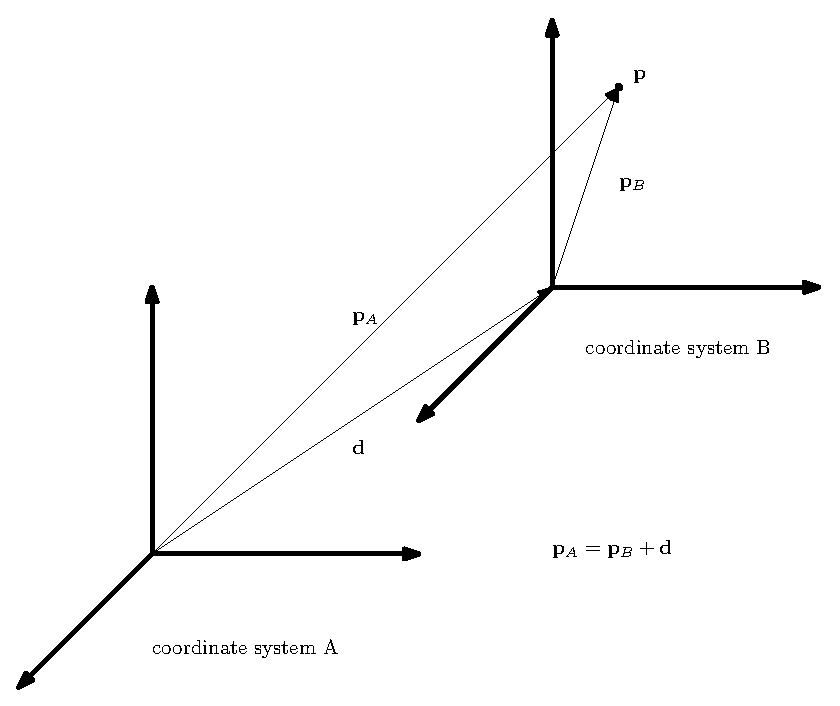
\includegraphics[width=12cm]{Math_transform/coordinateTranslate.eps}
    \caption{좌표계의 이동과 좌표의 변화}
    \label{fig:transform:coordinateTranslate}
\end{figure}

좌표계를 옮겨 놓는 변환을 $\mathbf T_{\mathbf d}$라고 하자.
이 변환은 다음 행렬로 표현된다.

$$
\mathbf T_{\mathbf d} = \left [
\begin{array}{cccc}
1 & 0 & 0 & d_x \\
0 & 1 & 0 & d_y \\
0 & 0 & 1 & d_z \\
0 & 0 & 0 & 1 \\
\end{array}
\right ]
$$

좌표는 다음과 같이 변환된다.

\begin{eqnarray}
\mathbf p_A = \mathbf T_{\mathbf d} \mathbf p_B \\ \nonumber
\mathbf p_B = \mathbf T_{\mathbf d}^{-1} \mathbf p_A \\ \nonumber
\end{eqnarray}

\subsection{좌표계의 회전}


\begin{figure}[h!]
  \centering
    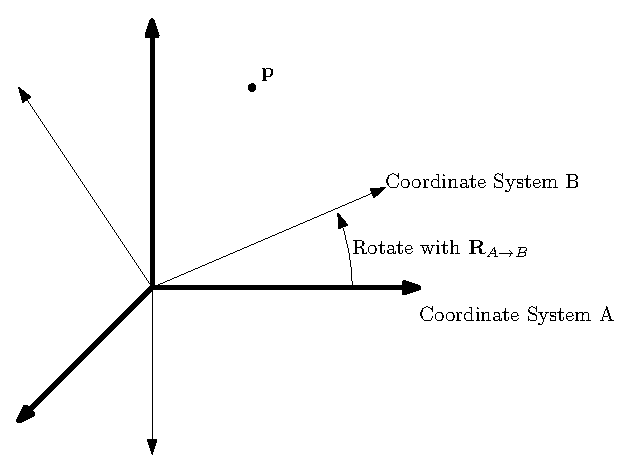
\includegraphics[width=8cm]{Math_transform/coordinateRotate.eps}
    \caption{좌표계의 회전}
    \label{fig:transform:coordinateRotate}
\end{figure}


이번에는 그림 \ref{fig:transform:coordinateRotate}와 같이 좌표계가 회전행렬 $\mathbf R_{A \rightarrow B}$에 의해 $A$에서 $B$로 회전되었다고 가정해 보자.
이 경우 각각의 좌표계를 기준으로 $\mathbf p$의 좌표를 정했을 때 얻어지는 좌표를 각각 $\mathbf p_A$와 $\mathbf p_B$라고 하자.
두 좌표 사이에는 다음과 같은 관계가 존재한다.

\begin{eqnarray}
\mathbf p_A &= \mathbf R_{A \rightarrow B} \mathbf p_B &\\ \nonumber
\mathbf p_B &=  \mathbf R_{A \rightarrow B}^{-1} \mathbf p_A & =  \mathbf R_{A \rightarrow B}^{\rm T} \mathbf p_A  \\ \nonumber
\end{eqnarray}


\subsection{회전과 이동이 함께 이뤄진 좌표계 변환}

\begin{figure}[h!]
  \centering
    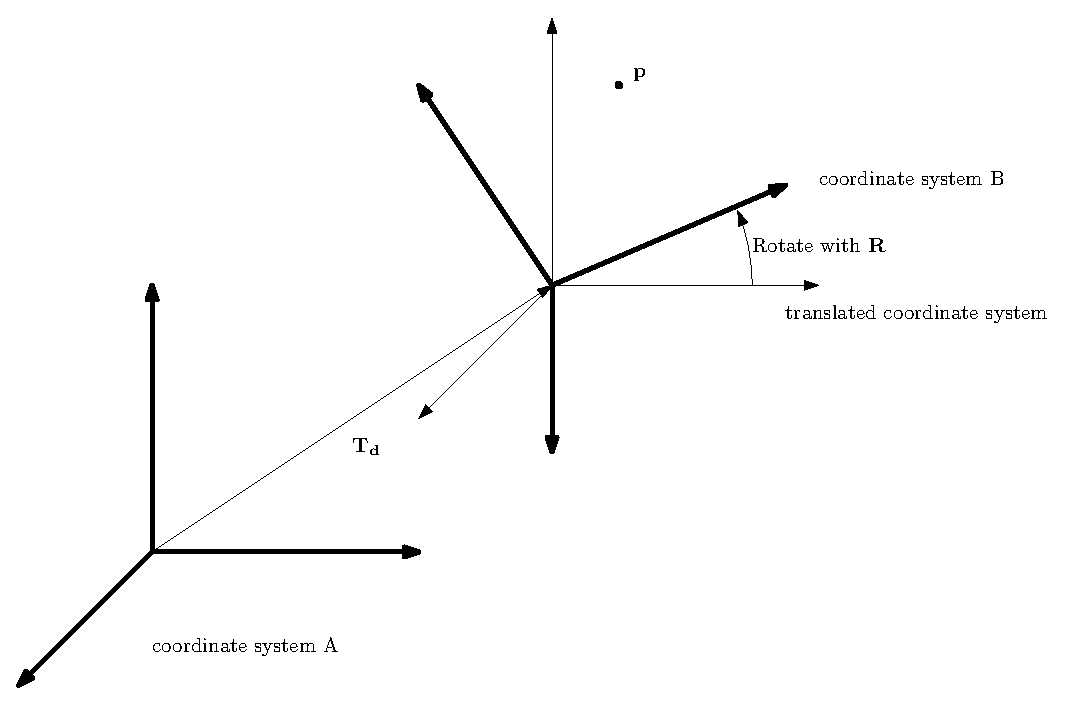
\includegraphics[width=12cm]{Math_transform/coordinateTransform.eps}
    \caption{좌표계의 회전}
    \label{fig:transform:coordinateTransform}
\end{figure}

이번에는 그림 \ref{fig:transform:coordinateTransform}와 같이 좌표계의 이동과 회전이 모두 이루어졌다고 가정해 보자.
이것은 좌표계를 $\mathbf R$로 회전한 뒤에 $\mathbf T_{\mathbf d}$를 이용하여 이동한 것이다.
회전행렬 $\mathbf R$과 이동변환행렬 $\mathbf T_{\mathbf d}$가 동차좌표계에서 정의되는 $4 \times 4$ 행렬이라면
둘은 다음과 같이 표현할 수 있다.

$$ 
\mathbf R = \left [ \begin{array}{cc} \mathbf R_{33} & 0 \\ \mathbf O_3^{row}  & 1 \end{array} \right ]
$$

$$ 
\mathbf T_{\mathbf d} = \left [ \begin{array}{cc} \mathbf I_{33} & \mathbf d \\ \mathbf O_3^{row} & 1 \end{array} \right ]
$$

회전이 먼저 이루어지고, 이동이 그 다음에 수행되므로 복합변환은 $\mathbf T_{\mathbf d} \mathbf R$가 된다.
그리고 이 행렬은 다음과 같다.

$$ 
\mathbf T_{\mathbf d} \mathbf R = \left [ \begin{array}{cc} \mathbf R_{33} & \mathbf d \\ \mathbf O_3^{row} & 1 \end{array} \right ]
$$

이때 좌표의 변환은 다음과 같다.



\begin{eqnarray}
\mathbf p_A &= 
\left [ \begin{array}{cc} \mathbf R_{33} & \mathbf d \\ \mathbf O_3^{row} & 1 \end{array} \right ]
\mathbf p_B &\\ \nonumber
\mathbf p_B &=  
\left [ \begin{array}{cc} \mathbf R_{33}^{\rm T} &  \mathbf R_{33}^{\rm T} \mathbf d \\ \mathbf O_3^{row} & 1 \end{array} \right ]
\mathbf p_A  \\ \nonumber
\end{eqnarray}
